\section{Etude de convergence}

\begin{figure}[!ht]
	\centering
	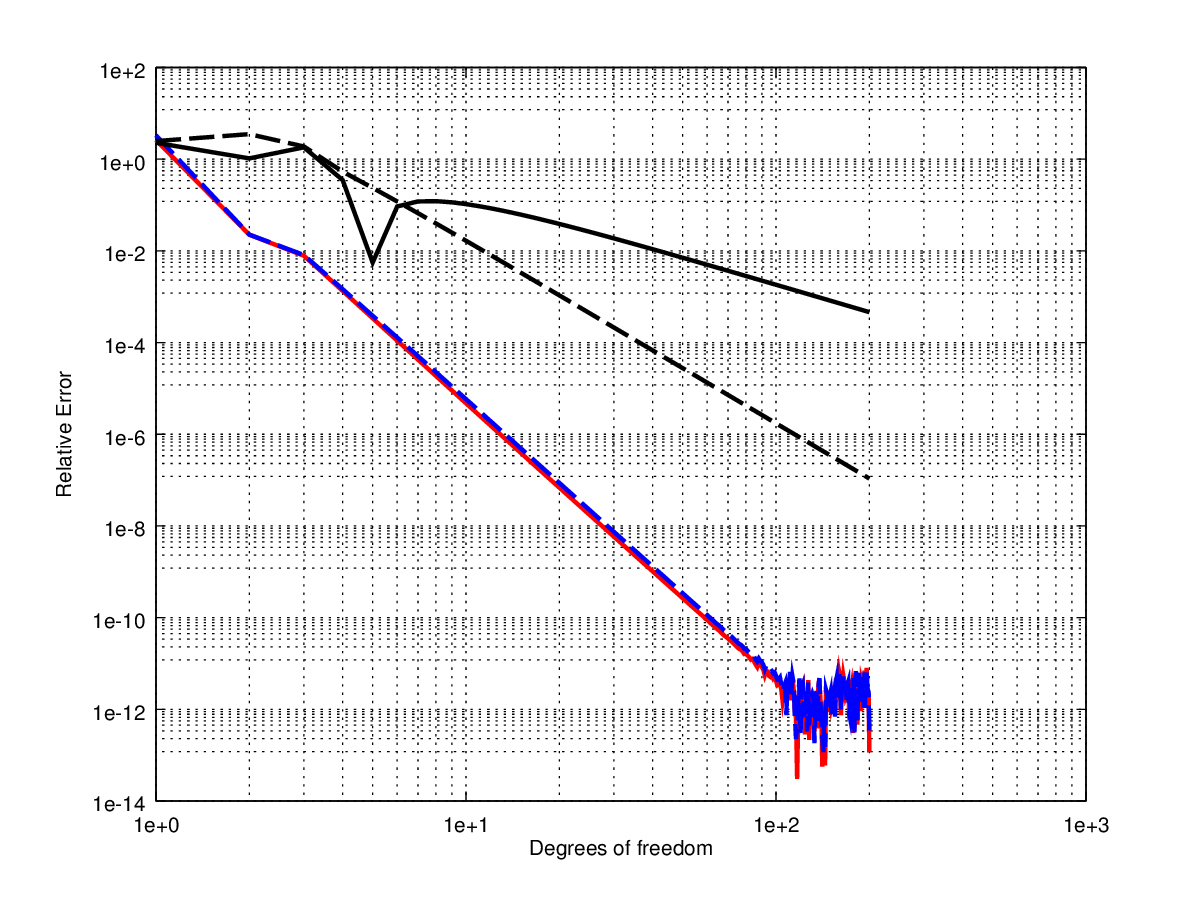
\includegraphics[width=11cm]{part4/figs/herm_comp.png}
	\caption{\label{fig:compp_quad_herm}Erreur relative commise avec des éléments quadratiques en noir (pointillés,
	méthode classique ; plein, méthode des caractéristiques) et avec des splines d'Hermite (en rouge et bleu).}
\end{figure}
